\documentclass[10pt,conference,compsocconf]{IEEEtran}

\usepackage{hyperref}
\usepackage{graphicx}	% For figure environment
\usepackage{color}
\usepackage{natbib}
\usepackage{float}
\usepackage{cprotect}
\usepackage{tabularx}
\usepackage{multirow}

\begin{document}
\title{Higgs Boson Challenge: Machine Learning Project}

\author{
  Robin Clerc, Pierre Vigier, Jacob Levy Abitbol\\
  \textit{Master of Computer Science, EPFL, Switzerland}
}

\maketitle

\begin{abstract}
  The CERN produces petabytes of data each day on the base of the ATLAS project, leading the research on the Higgs boson's decay.The often complex and high dimensional data sets generated in experiments are often hard to analyze and interpret. We give here an overview on how different learning methods perform on a collision event dataset.
  \end{abstract}

\section{Introduction}

The Higgs Boson is an elementary particle which explains why other particles have mass. It was discovered in collision experiments in the LHC, where proton bunches are accelerated on a circular trajectory in both directions. The collisions between the protons are detected by sensors of the ATLAS detector which also detect particles resulting from those collisions, resulting in the real-valued variables which we are provided with. These sensors however detect either actual interesting events or uninteresting events. The end goal of this project is then to improve the classification of the signal / background events, given the real-valued features resulting from the collision event.

\section{Models and Methods}
\label{sec:structure-paper}

\subsection{Data Exploration and Preprocessing}
The provided training dataset consists of a 250K samples corpus of collision events, where each event is classified as either signal $S$ or background $B$. Each collision is characterized by a set of 30 features from which the predictions will be made. A separate test set of unlabelled samples on which to test the performance of our models is also provided. \\
A first glance at our dataset reveals that overall,
more than 70\% of the events lack at least one feature, which is indicated in the data  by the value $-999$. These have to be imputed in order to be able to feed our dataset to a learning method. To handle this missing information we replaced the missing values of a given feature by its mean value, calculated separately for the training and the test set. \\
We also noticed that 12 out of the 30 available features included in the dataset seem to be power-law distributed. In order to compensate for the high skew of the observed distributions, we took the logarithm of these selected features instead of the actual features themselves (see Figure \ref{fig_kde}).\\ Each feature was then normalized using the means and standard deviations computed over the training set. 

\begin{figure}[htb]
\centering
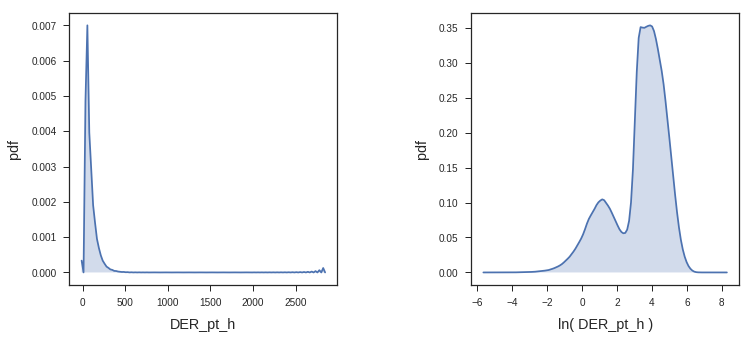
\includegraphics[width=0.8\linewidth]{kdeplot.png}

\cprotect\caption{KDE plot for the modulus of the vector sum of the transverse momentum of the hadronic tau \verb+DER_pt_h+.
\emph{Left}: Original distribution. \emph{Right}:  Distribution of log values}
\label{fig_kde}
\end{figure}

%12 features take their values in a range describing several orders of magnitude in the positive values and with very sparse density in the high values.

The \verb+PRI_jet_num+ feature (a jet is a particle) is interesting because our correlation study highlights a very high correlations between features containing -999 values. Indeed -999 values are not actually features that sensors failed to catch, it is simply that they do not exist : if there is no jet, it has no speed, or if there is 1 jet we cannot compute any angle between jets. We can split those sets in 3 categories not having the same number of initial features.
\vspace{-0.1cm}
\begin{figure}[H]
\centering
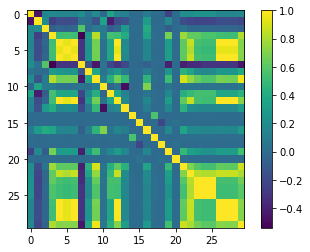
\includegraphics[width=0.6\linewidth]{corr.png}
\cprotect\caption{Pairwise correlations of base features. Labels indicate the feature's index in the provided dataset. }
\label{fig_corr}
\end{figure}

An additional exploratory analysis via the pairwise correlation matrix (cf Figure \ref{fig_corr}) reveals a clear cutoff between primitive and derivative features (starting around index 14) where  primitive features are highly correlated among themselves.¡

We also took notice that the \verb+PRI_jet_num+ feature, representing the number of particles or jets generated from the collision takes only 4 integer values (ranging from 0 to 3). This allowed to reduce the dimensionality of the original feature space by splitting our learning problem into 3 separate ones, each for a specific value of the number of jets (0,1,2-3).\\
This in turn enabled us to further remove static features from the dataset, yielding 19 features for  \verb+Jet 0+, 23 for \verb+Jet 1+ and 30 for \verb+Jet 2-3+ (see Table \ref{tab_feats})
\begin{table}[h!]
\centering
\caption{Missing values per feature and per jet value shown for features containing NaN (*: all, /: None)}
\footnotesize
\hspace{-0.2cm}
\begin{tabular}{ l| ccc } 
 \hline
   NaN Features & Jet 0 & Jet 1 & Jet 2-3 \\
 \hline
   \verb+DER_deltaeta_jet_jet+  & * & * & /  \\
   \verb+DER_lep_eta_centrality+  & * & / & / \\
   \verb+DER_mass_jet_jet+  & * & * & / \\
   \verb+DER_prodeta_jet_jet+  & * & * & /  \\ 
   \verb+PRI_jet_all_pt+  & * & * & /  \\
   \verb+PRI_jet_leading_eta+  & * & * & / \\
   \verb+PRI_jet_leading_phi+  & * & / & /   \\
   \verb+PRI_jet_leading_pt+  & * & / & / \\
   \verb+PRI_jet_subleading_eta+  & * & / & / \\
   \verb+PRI_jet_subleading_phi+  & * & * & /  \\
   \verb+PRI_jet_subleading_pt+  & * & * & /  \\
  \hline
\end{tabular}
\label{tab_feats}
\end{table}

Finally, the difference of the particle azimuthal angles $\Phi$, namely, \verb+PRI_tau_phi+, \verb+PRI_lep_phi+, \verb+PRI_met_phi+, were considered to be of potential interest  in determining the nature of the collision detected and were therefore added as features. \\
Also, we found interesting to introduce non-linearities in our dataset by adding to our original data the  polynomial values of the features with degree less than or equal to $n$. This was then expanded to include the polynomial combinations of the features up to degree $M=\sqrt{n}$. This allows to keep a decent proportion of cross as the degree $n$ of the base features increases.\vspace{-0.25cm}


\section{Results and Discussion}
As shown, in Table \ref{tab_first_run}, the use of the more sophisticated Newton based  gradient descent methods was hindered by the the non-invertible nature of the Hessian matrix. Instead of implementing quasi-Newton methods to work around this condition, we chose to focus on the three first models. Also, the gradient descent using the SGD variant with a batch size of 256 training samples due to the high number of samples and features that were studied jointly. The models parameters were arbitrarily set at first at  $\lambda_=10^{-3}$,$\gamma=2.10^{-5}$, \verb+max_iter+=5000. 
\begin{table}[h!]
\centering
\caption{Initial training results (Model predictive accuracy \%)}
\footnotesize
\hspace{-0.3cm}
\begin{tabular}{ l| ccc } 
 \hline
   Model & \verb+Jet 0+& \verb+Jet 1+& \verb+Jet 2-3+ \\
 \hline
   \verb+linear_regr+  & 82.56 &74.18  & 77.68  \\
   \verb+ridge_regr+  & 82.50 & 74.17  & 77.67 \\
   \verb+log_regr_gd+ & 81.23 & 72.54  & 79.35\\
   \verb+penal_log_regr_gd+  &  83.03  &  76.82 & 81.27 \\ 
   \verb+log_regr_newton+  & / & / & / \\
   \verb+penal_log_regr_newton+ &  / & / & / \\
  \hline
\end{tabular}
\label{tab_first_run}
\end{table}
We observed that the baseline application of the learning algorithms already provided good performances with accuracy scores ranging from 74\% to 83\%, the lowest accuracy corresponding to the \verb+Jet 1+ group. Given the small gain (from 1 \% to 2\%) obtained from using logistic regression models with respect to using simpler linear models as well as the higher parametrization cost of the logistic models (in terms of definition and training), we chose to focus on linear regression to train our classifier using either Least Squares or Ridge Regression.
We proceeded to compare the performance of these two  different learning algorithms by using a grid search with either a 4- or 10- fold cross-validation on the model's parameters: 

\subsection{Least squares}
This model, when trained using its closed-formed solutions (depending on whether or not the Gram matrix is invertible), is parameter-free. We needed only to choose the degree  up to which the polynomial features will be calculated. The optimal degree was obtained by grid-searching different values of $n$ ranging from 1 to 16 for each \verb+Jet+: 
\vspace{-0.2cm}
\begin{table}[h!]
\centering
\caption{LS gridsearch with (MOI) and without $M^{th}$-order interactions  }
\footnotesize
\begin{tabular}{|l| c|c| } 
 \hline
   Jet & Degree & 10-fold Accuracy (\%)  \\
 \hline
    \verb+Jet 0+  & 8 &  84.18 \\
    \verb+Jet 0 (MOI)+   & 10 &  84.31 \\
    \verb+Jet 1+  & 4 & 79.13 \\
    \verb+Jet 1 (MOI)+  & 9 & 79.56 \\
    \verb+Jet 2-3+  & 9 & 81.25\\
    \verb+Jet 2-3 (MOI)+ & 9 & 81.97\\
  \hline
\end{tabular}
\label{grid_search_ridge_cross}
\end{table}
As can be observed in the above table, we clearly see that the adding of the polynomial features and the $M^{th}$-order interaction terms proved beneficial in terms of our model's predictive power, as the accuracy was raised consistently across different jets from $2\%$ in \verb+Jet 0+  to $5\%$ in \verb+Jet 1+. In spite of the small accuracy increase achieved by the addition of the \verb+MOI+, these were kept in what follows. Using high order terms led to overfitting during training which drove us to try penalizing high weights via Ridge regression. 
\subsection{Ridge regression}
The optimal parametrization of this model required us to grid-search over the degree of the polynomial to be applied as well as the $\lambda$ regularization term to penalize high values for the weights. The $\lambda$ parameter was sampled uniformly from $[10^{-20},10^{-3}]$ and the degree $n$ was considered as in the previous case: 
\vspace{-0.5cm}
\begin{table}[h!]
\centering
\caption{Ridge regression grid search  with  $M^{th}$-order interactions}
\footnotesize
\begin{tabular}{|l| cc|c| } 
 \hline
   Jet & Degree & Lambda & 10-fold Accuracy (\%)  \\
 \hline
   \verb+Jet 0+  & 11 & $10^{-15}$  & 84.59  \\
   \verb+Jet 1+  & 12 & $10^{-15}$  & 80.25 \\
   \verb+Jet 2-3+  & 14  &  $10^{-13}$ & 82.62 \\
  \hline
  \end{tabular}
\label{grid_search_ridge_cross}
\end{table}

Although modest, we find consistently greater performances across all different \verb+Jet+ values when adding the Tikhonov regularization term. It is worth noticing that, even with a small regularization term, this model allows for the adding of higher order polynomial features than least square without it leading necessarily to overfitting the training set. 


\section{Conclusion}
Classification tasks on complex datasets call for the use of different learning models to perform prediction. In this project a ridge regression model was implemented to classify detected collision events at CERN as signal or background. By preprocessing the data and grid-searching the best parameters , we acheived an accuracy of -\%. Several other approaches in the preprocessing and the model choice might have lead to greater scores such as using LASSO regularization, reducing the dimension of the dataset with a PCA, or interpolating the missing features values from the present ones.

\end{document}
\subsection{Data preprocessing}

As previously stated, we split the sets in 3 categories:  
\begin{itemize}
    \item $Jet0$ for which we exclude the 12 constant features
    \item $Jet1$ for which we exclude the 8 constant features
    \item $Jet{2;3}$ 
\end{itemize}

We log-transform the features taking their values in several orders of magnitude.

The we standardize each category by :
\begin{itemize}
    \item Getting the mean and the standard deviation of the training set category.
    \item Normalize the training set category
    \item Normalize the test set category with the mean and standard deviation of the training set.
\end{itemize}

\subsection{Feature engineering}

 First of all, as we are provided with angles, it can be interesting to add as a feature the absolute differences between those angles to extract more information.








